\documentclass{article}
\usepackage[utf8]{inputenc}
\usepackage{graphicx}
\usepackage{hyperref}
\usepackage{geometry}
\geometry{a4paper} % Set the page size to A4
\usepackage{listings} % Package for including code in the document

\title{Práctica 06: Creación de una base de datos}
\author{Carlos I. Padilla Herrera}
\date{12 de mayo de 2024}

\lstset{frame=single, % Adds a frame around the code
        basicstyle=\small\ttfamily, % Use a small, true type font
        language=SQL, % SQL syntax highlighting
        showstringspaces=false} % Don't mark spaces in strings

\begin{document}

\begin{titlepage}
    \centering
    \vspace*{1cm}
    \Huge\textbf{Curso de base de datos entre semana G0224}
    
    \vspace{0.5cm}
    \LARGE Escuela de Código PILARES
    
    \vspace{1.5cm}
    \textbf{Carlos Ignacio Padilla Herrera}
    
    \vspace{2cm}
    \Large\textbf{Folio:} 794DR02
    
    \vspace{0.5cm}
    \Large\textbf{Práctica 6:} Creación de una base de datos.
    
    \vfill
    
    \Large\textbf{Fecha:} 13 de mayo de 2024
    
    \vspace{0.8cm}
\end{titlepage}

\newpage

\section*{Código SQL para la creación de tablas y inserción de datos}

\begin{lstlisting}
-- Creating tables
create table manufacturer (
    code int(10) primary key,
    name varchar(100)
);

create table product (
    code int(10) primary key,
    name varchar(100),
    price double,
    manufacturer_code int(10),
    foreign key (manufacturer_code) references manufacturer(code)
);

-- Inserting manufacturers
insert into manufacturer (code, name) values
(1, 'Asus'),
(2, 'Lenovo'),
(3, 'Hewlett-Packard'),
(4, 'Samsung'),
(5, 'Seagate'),
(6, 'Crucial'),
(7, 'Gigabyte'),
(8, 'Huawei'),
(9, 'Xiaomi');

-- Inserting products
insert into product (code, name, price, manufacturer_code) values
(1, 'Disco Duro SATA3 1TB', 86.99, 5),
(2, 'Memoria RAM DDR4 8GB', 120, 6),
(3, 'Disco SSD 1TB', 150.99, 4),
(4, 'GeForce GTX 1050 Ti', 185, 7),
(5, 'GeForce GTX 1080 Xtreme', 755, 6),
(6, 'Monitor 24 LED Full HD', 202, 1),
(7, 'Monitor 27 LED Full HD', 245.99, 1),
(8, 'Portatil Yoga 520', 559, 2),
(9, 'Portatil Ideapad 320', 444, 2),
(10, 'Impresora HP Deskjet 3720', 59.99, 3),
(11, 'Impresora HP Laserjet Pro M26nw', 180, 3);
\end{lstlisting}

\newpage % Inicia una nueva página

\section*{Captura de pantalla}

\begin{figure}[ht]
    \centering
    \href{https://www.db-fiddle.com/f/nF3pqUTYuEuymCCpV78uN/1}{
        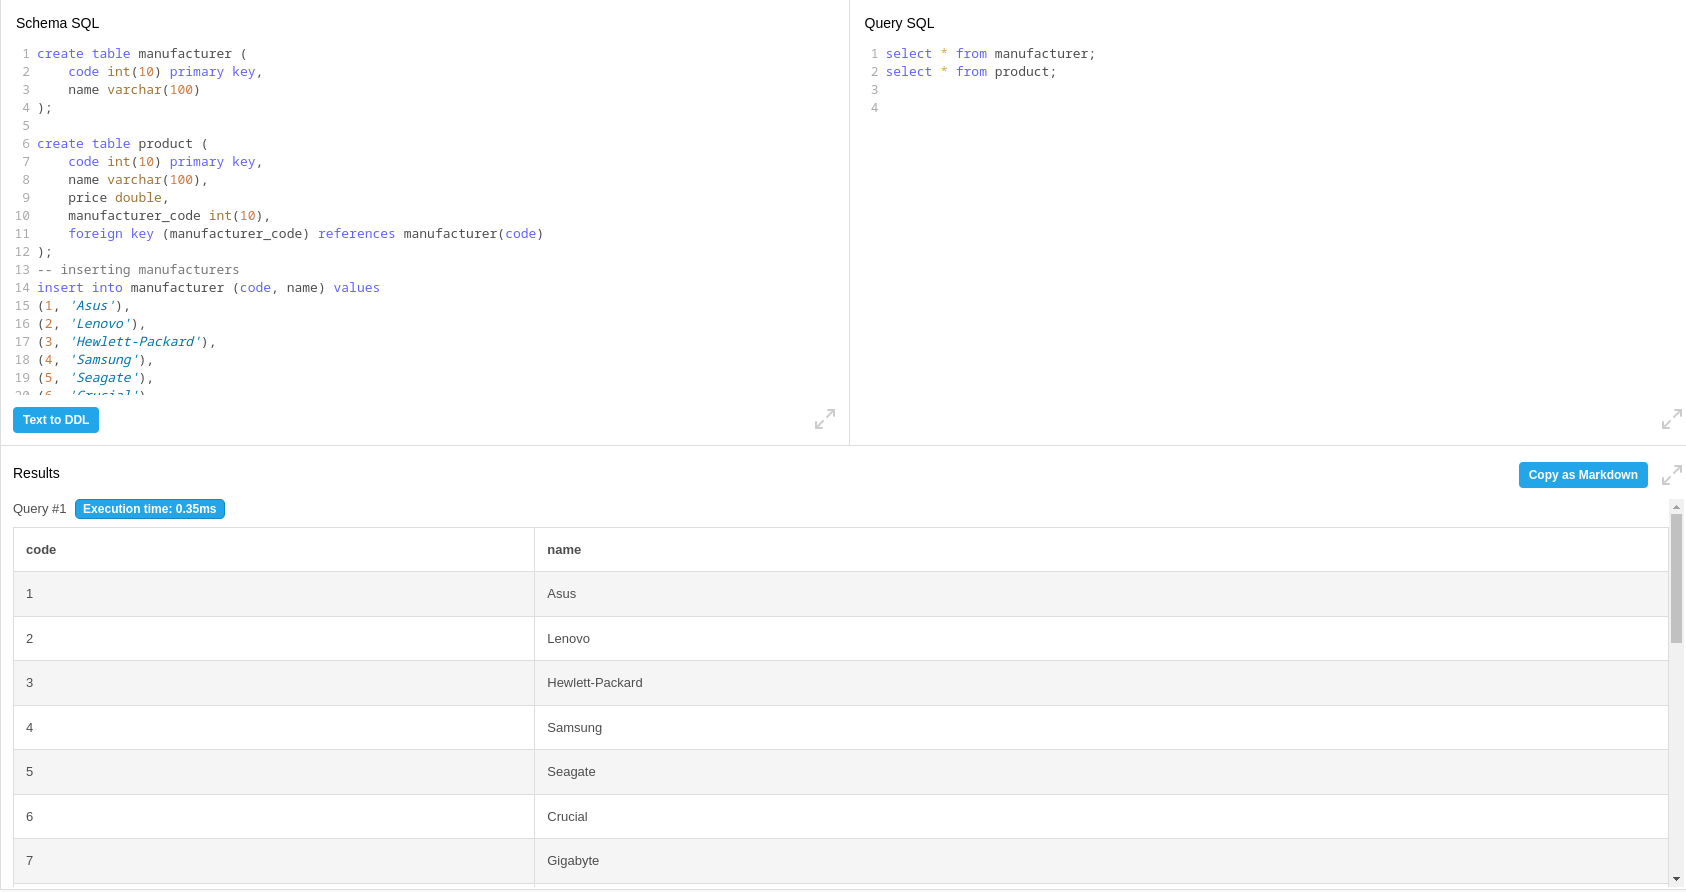
\includegraphics[width=\linewidth]{screenshot.png} % Asegúrate de que el nombre del archivo y la extensión son correctos
    }
    \caption{Captura de pantalla que te dirige a DB Fiddle con el código si le das click.}
\end{figure}


\end{document}
